\documentclass[10pt]{article}
\usepackage[utf8]{inputenc}
\usepackage[doublespacing]{setspace}
\usepackage{textcomp}
\usepackage{amsmath,amssymb,amsthm}
\usepackage{fancyhdr}
\usepackage{lastpage}
\usepackage[]{hyperref}
\usepackage[pdftex]{graphicx}
\usepackage{ctex}
\usepackage{booktabs}
\usepackage{subfigure}
\usepackage{titlesec}
\usepackage{listings}
\usepackage{enumerate}
\usepackage{bm}
\usepackage{float}
\usepackage{verbatim}
\usepackage{multirow}
%\allowdisplaybreaks
\renewcommand{\contentsname}{\centerline{Contents}}
\pagestyle{fancy}
\author{D; D}
\def\name{D; D}
\lhead{Data Mining}
\chead{}
\rhead{\name}
\cfoot{-\space\thepage\space-}
\newtheorem{exer}{\bm{$Exercise$}}
\newtheorem{prob}{\bm{$Problem$}}
\newtheorem{bonus}{\bm{$Bonus\;Problem$}}
\newcommand{\tabincell}[2]{\begin{tabular}{@{}#1@{}}#2\end{tabular}}
\CTEXoptions[today=old]

\begin{document}

\title{Assignment Three}
\date{\today}
\maketitle
\thispagestyle{fancy}
\thispagestyle{fancy}

\begin{prob}
\end{prob}
\begin{enumerate}[1)]
\vspace{3mm}

\item
R codes:
\lstinputlisting{p11a.R}
R outputs:
\lstinputlisting{p11a.txt}
\begin{figure}[H]
  \centering
  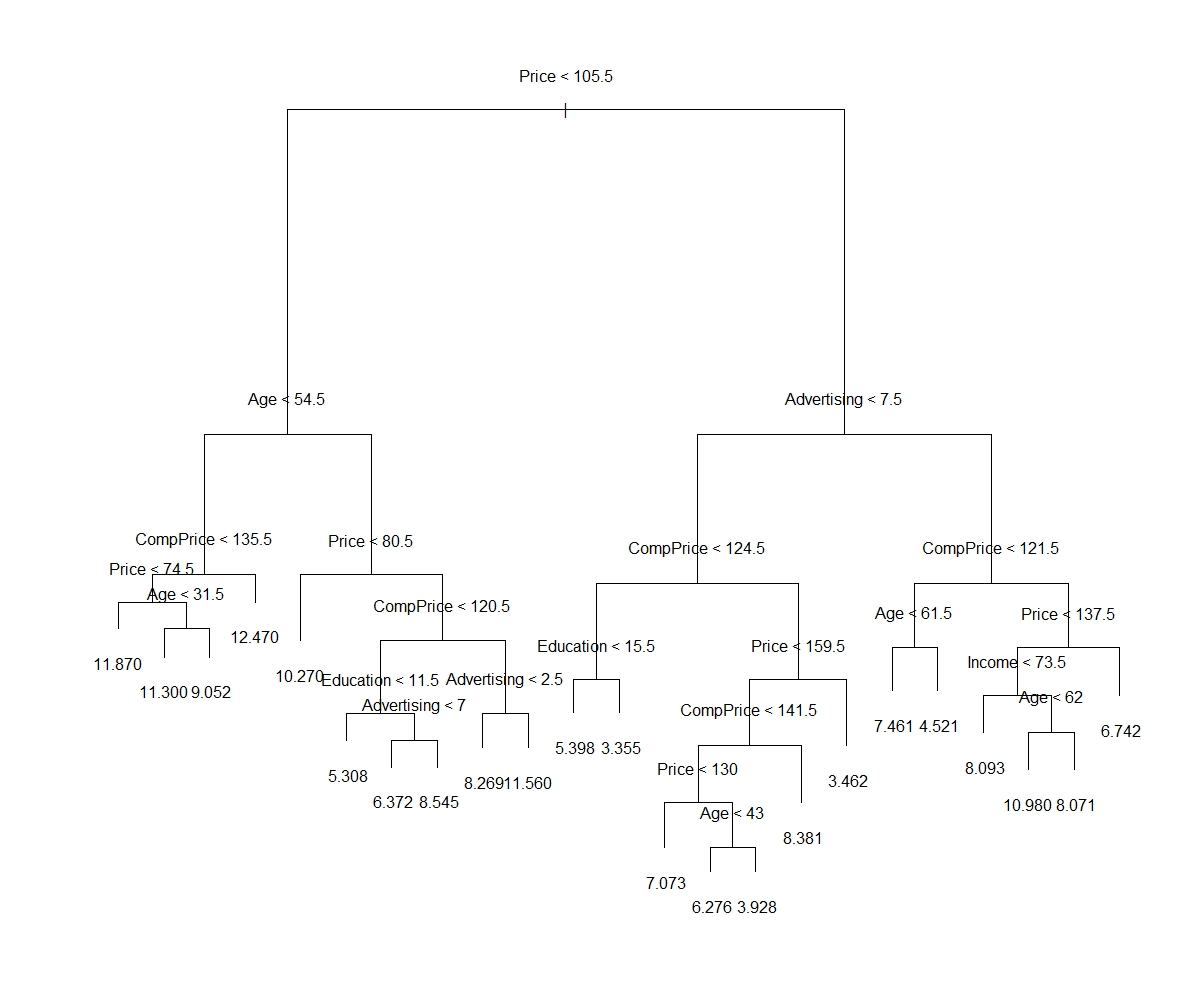
\includegraphics[width=12cm,height=10cm]{p11a.jpeg}
  \caption{The regression tree for the car seat data}
\end{figure}
Interpretations:\\
For the car seat data, Figure 1 is a regression tree for predicting the sales of a car, based on the variables the comparable price, the income, the advertising, the price, the age, and the education. At a given internal node, the label (of the form $X_j<t_k$) indicates the left-hand branch emanating from that split, and the right-hand branch corresponds to $X_j>t_k$. For example, the split at the top of the tree results in two large branches. The left-hand branch corresponds to $Price<105.5$, and the right-hand branch corresponds to $Price\geq105.5$. The tree has 22 internal nodes and 23 terminal nodes. The number in each leaf is the mean of the response for the observations that fall there.\footnote{ James, G., Witten, D., Hastie, T., \& Tibshirani, R. (2014). \textit{An introduction to statistical learning with applications in R}. Springer, 304.} The residual mean deviance is 3.296. The residuals of the minimum, the first quarter, the median, the mean, the third quarter and the maximum are -4.994, -1.178, 0.037, 0.000, 1.390 and 4.627 respectively.\\

MSEs:\\
R codes:
\lstinputlisting{p11b.R}
R outputs:
\lstinputlisting{p11b.txt}
The MSE for the training data set is 3.043394; the MSE for the testing data set is 6.03393.
\vspace{3mm}

\item
We use 5-fold cross validation ($K=5$), which means 20\% of the data is used for testing and is usually accurate.\footnote{ JahKnows. (2018). \textit{Answer to how to calculate the fold number (k-fold) in cross validation}. Retrieved from \url{https://datascience.stackexchange.com/questions/28158/how-to-calculate-the-fold-number-k-fold-in-cross-validation}.}\\
R codes:
\lstinputlisting{p12a.R}
R outputs:
\lstinputlisting{p12a.txt}
\begin{figure}[H]
  \centering
  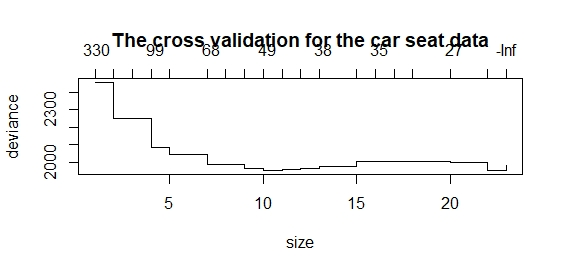
\includegraphics[width=8cm,height=5cm]{p12a.jpeg}
  \caption{The cross validation for the car seat data}
\end{figure}
Based on the outputs, we choose $size=11$.\\
R outputs:
\begin{figure}[H]
  \centering
  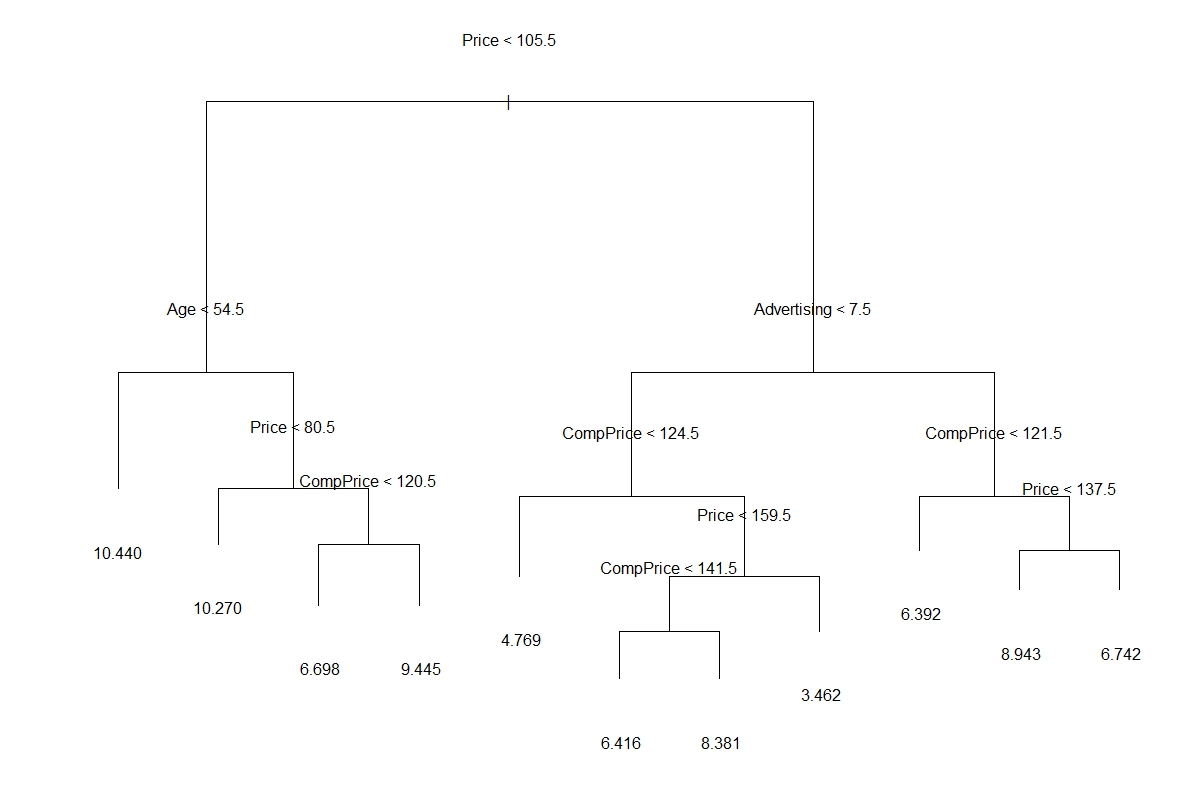
\includegraphics[width=12cm,height=8cm]{p12b.jpeg}
  \caption{The pruned regression tree for the car seat data}
\end{figure}
\lstinputlisting{p12b.txt}
According to the new MSEs, 4.38325 for the training and 6.05599 for the testing, both greater than those for the original regression tree. The pruned tree does not perform better.
\vspace{3mm}

\item
Fit a bagged regression tree:\\
R codes:
\lstinputlisting{p13a.R}
R outputs:
\lstinputlisting{p13a.txt} % Comment: identical code?
According to the new MSEs, 0.8515121 for the training and 4.442605 for the testing, both smaller than those for the original regression tree. The bagged tree performs better.
\vspace{3mm}

Fit a random forest:\\
R codes:
\lstinputlisting{p13b.R}
R outputs:
\lstinputlisting{p13b.txt} % Comment: identical code?
\begin{figure}[H]
  \centering
  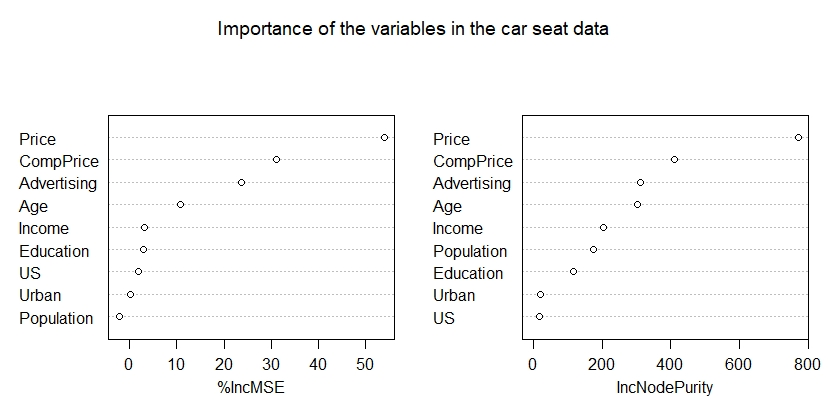
\includegraphics[width=10cm,height=6cm]{p13a.jpeg}
  \caption{Importance of the variables in the car seat data}
\end{figure}
According to the new MSEs, 0.894485 for the training and 4.34613 for the testing, both smaller than those for the original regression tree. The random forest performs better.\\
In all, the decorrelating trees were an effective strategy for this problem. % Comment: Is it better than bagging though?
\vspace{3mm}

\item
Fit a boosted regression tree:\\
R codes:
\lstinputlisting{p14a.R}
R outputs:
\lstinputlisting{p14a.txt}
\begin{figure}[H]
  \centering
  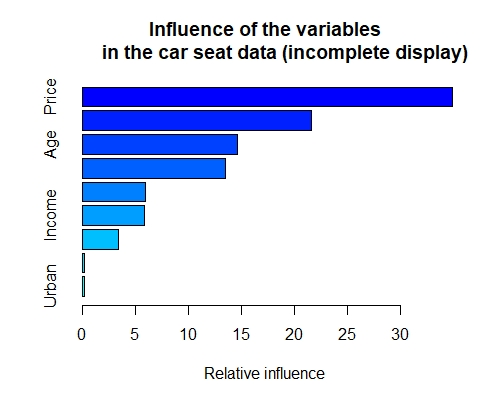
\includegraphics[width=9cm,height=7cm]{p14a.jpeg}
  \caption{Influence of the variables in the car seat data (incomplete display)}
\end{figure}
After several attempts, with the results from cross-validation, we find our best boosted regression tree:\\
R codes:
\lstinputlisting{p14b.R}
R outputs:
\lstinputlisting{p14b.txt} % Comment: This is worse than the first one you fitted! (for boosting)
\begin{figure}[H]
  \centering
  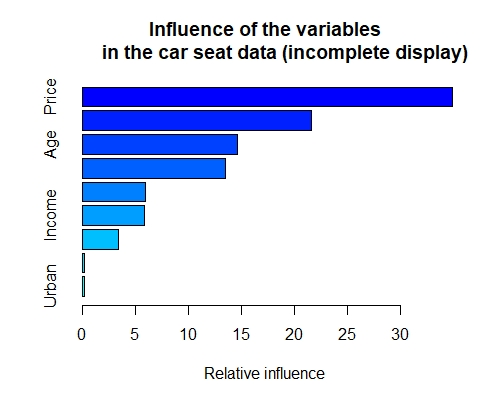
\includegraphics[width=9cm,height=7cm]{p14a.jpeg}
  \caption{Influence of the variables in the car seat data (incomplete display)}
\end{figure}
According to the new MSEs, 2.927084 for the training and 3.963599 for the testing, both smaller than those for the original regression tree. The boosted tree (tree depth = 1, shrinkage parameter = 0.1 and number of trees = 320) performs better.
\vspace{3mm}

Comments:\\
We use the following parameters, with the tree depth being 1, the shrinkage parameter being 0.1 and the number of trees being 320.\\
We get the top 7 variables based on the descending influence, which are the price, the comparable price, the age, the advertising, the income, the population and the education. The price is the most influential variable to the car sales; the urban and the US play very small role in the car sales.\\
The boosted tree performs better than the original regression tree. Especially, it gets the lowest MSE for the testing data, so this tree is the best so far to predict with the testing data.
\vspace{3mm}

\item
In all, based on the MSEs, the boosted tree (tree depth = 1, shrinkage parameter = 0.1 and number of trees = 320) performs the best in our work, and the most important predictor is the price in this model. % Comment: Any other predictors important?

\end{enumerate}
\vspace{3mm}

\begin{prob}
\end{prob}
\begin{enumerate}[1)]
\vspace{3mm}

\item
The nodes are labelled.
\begin{figure}[H]
  \centering
  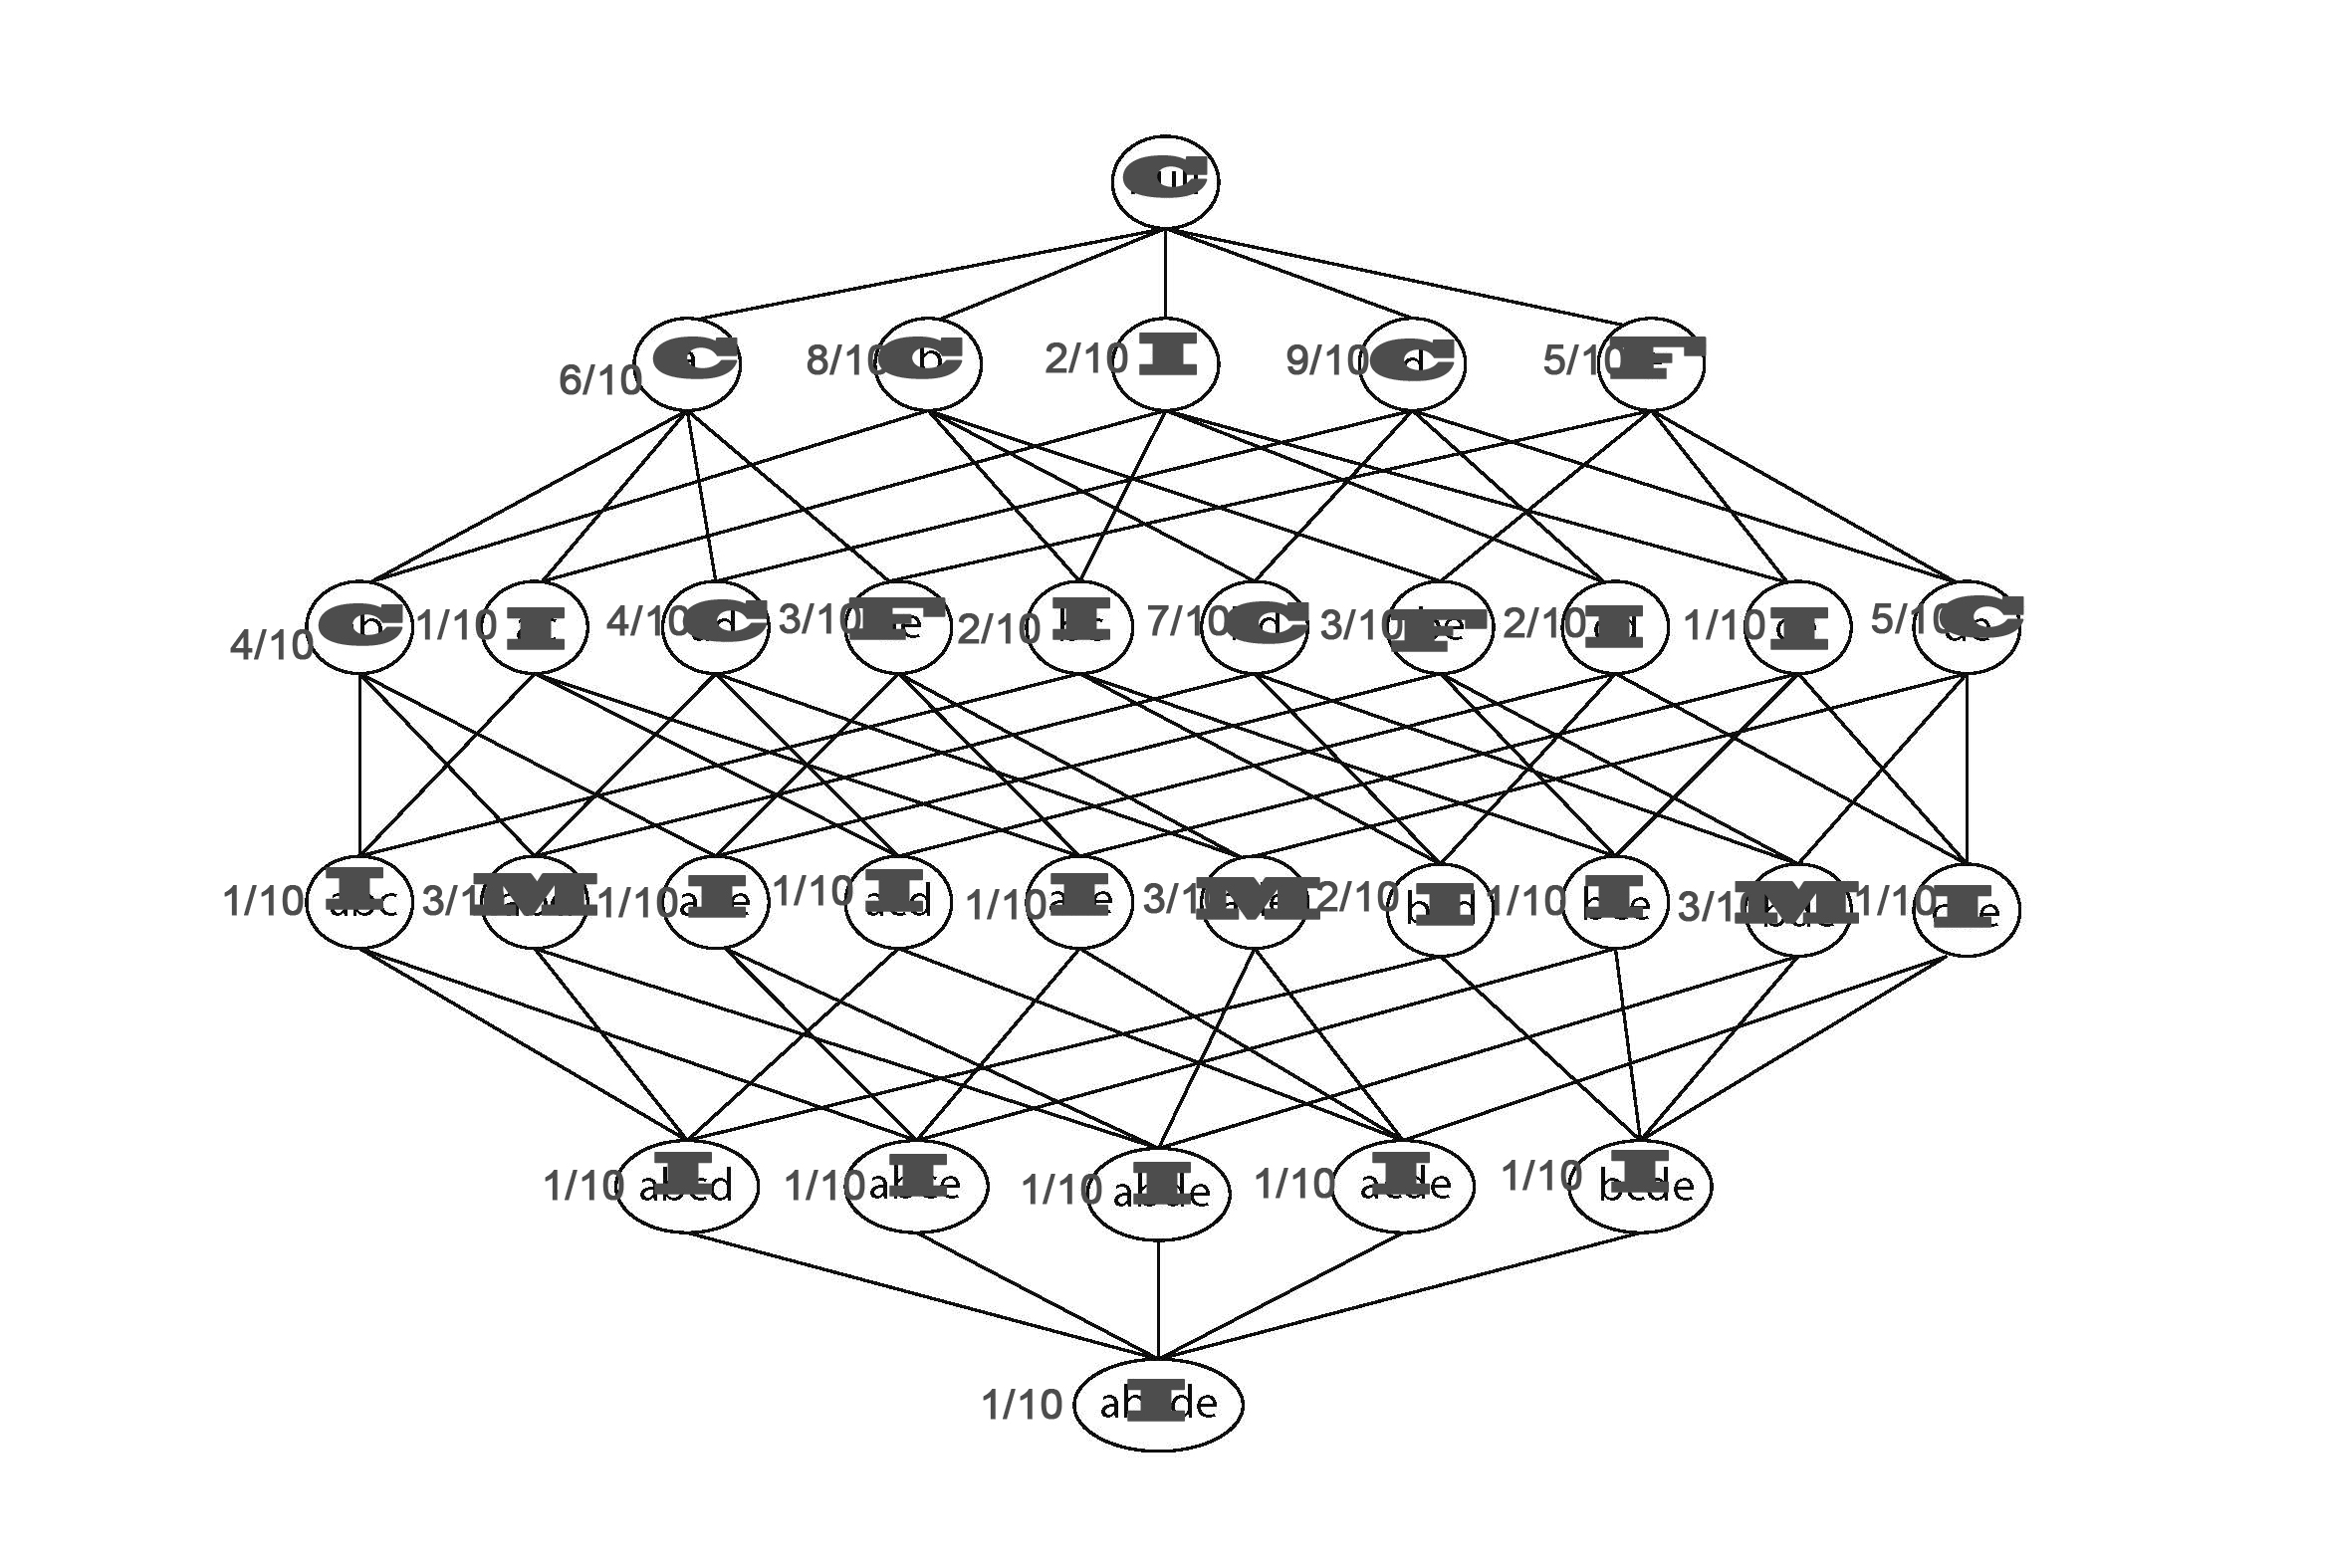
\includegraphics[width=12cm,height=10cm]{p21a.jpg}
  \caption{The supports (on the left of each node) and the labels (inside each node), where $label\in\{M,C,F,I\}$)} % Comment: C x; M -> M, C; M -> C; M -> C
\end{figure}
\vspace{3mm}

\item
We have the confidence defined as
\begin{align*}
conf(\{d,e\}\to\{b\})&=\frac{supp(\{d,e\}\cup\{b\})}{supp(\{d,e\})}\\
&=\frac{P(\mathbb{E}[\{d,e\}]\cap\mathbb{E}[\{b\}])}{\frac{5}{10}}\\
&=\frac{\frac{3}{10}}{\frac{5}{10}}\\
&=\frac{3}{5}
\end{align*}
We have the lift defined as
\begin{align*}
lift(\{d,e\}\to\{b\})&=\frac{supp(\{d,e\}\cup\{b\})}{supp(\{d,e\})supp(\{b\})}\\
&=\frac{conf(\{d,e\}\to\{b\})}{supp(\{b\})}\\
&=\frac{\frac{3}{5}}{\frac{8}{10}}\\
&=\frac{3}{4}
\end{align*}
Comments:\\
The rule $\{d,e\}\to\{b\}$ has a confidence of 0.6 in the database, which means that for 60\% of the transactions containing $\{d,e\}$ the rule is correct; in other words, 60\% of times a customer buys $\{d,e\}$, $\{b\}$ is bought as well.\\
The rule $\{d,e\}\to\{b\}$ has a lift of 0.75 in the database, which means that the items $\{d,e\}$ and $\{b\}$ are substitute to each other. This means that presence of $\{d,e\}$ has negative effect on presence of $\{b\}$ and vice versa.\footnote{ Wikipedia contributors. (2019). Association rule learning. \textit{Wikipedia, the free encyclopedia}. Retrieved from \url{https://en.wikipedia.org/w/index.php?title=Association_rule_learning&oldid=919694948}.}

\end{enumerate}
\vspace{3mm}

\begin{prob}
\end{prob}
\begin{enumerate}[1)]
\vspace{3mm}

\item
R codes:
\lstinputlisting{p31a.R}
R outputs:
\lstinputlisting{p31a.txt}
\begin{figure}[H]
  \centering
  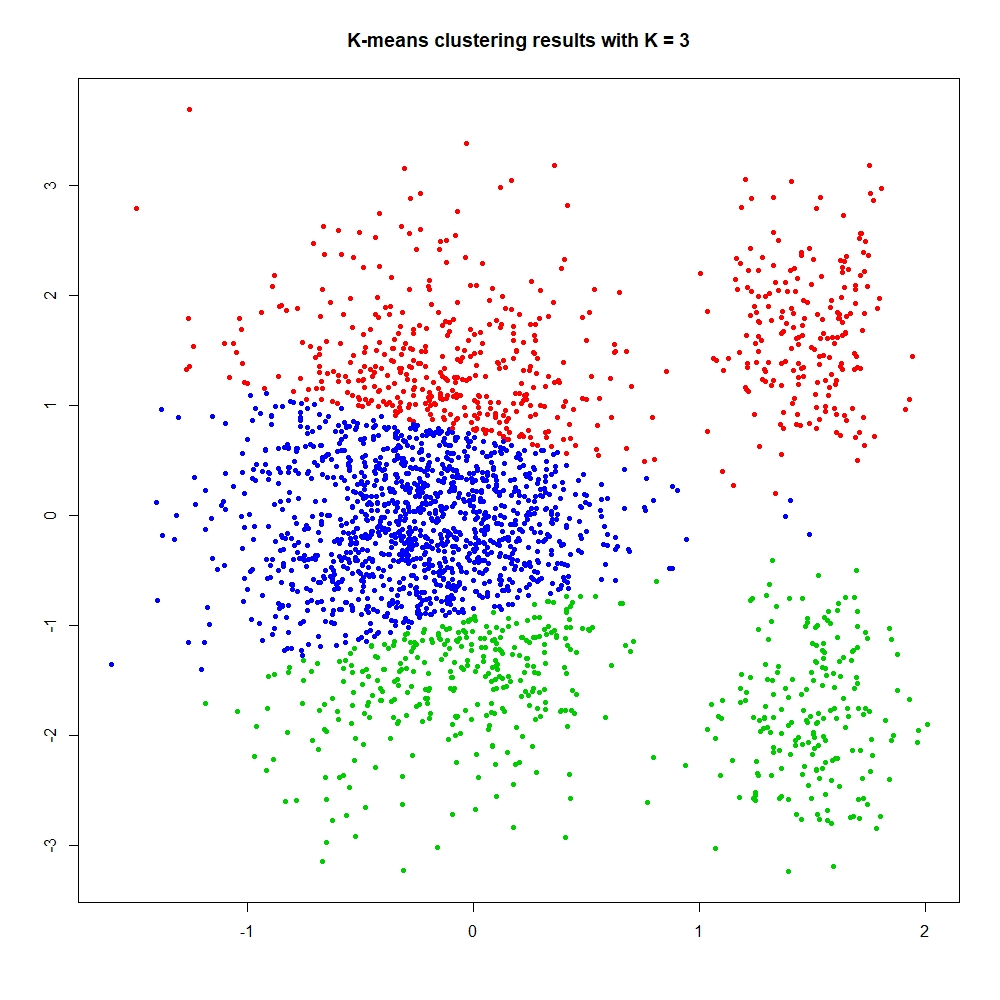
\includegraphics[width=9cm,height=9cm]{p31a.jpeg}
  \caption{K-means clustering results ($K=3$)}
\end{figure}

\item
R codes:
\lstinputlisting{p32a.R}
R outputs:
\lstinputlisting{p32a.txt}
\begin{figure}[H]
  \centering
  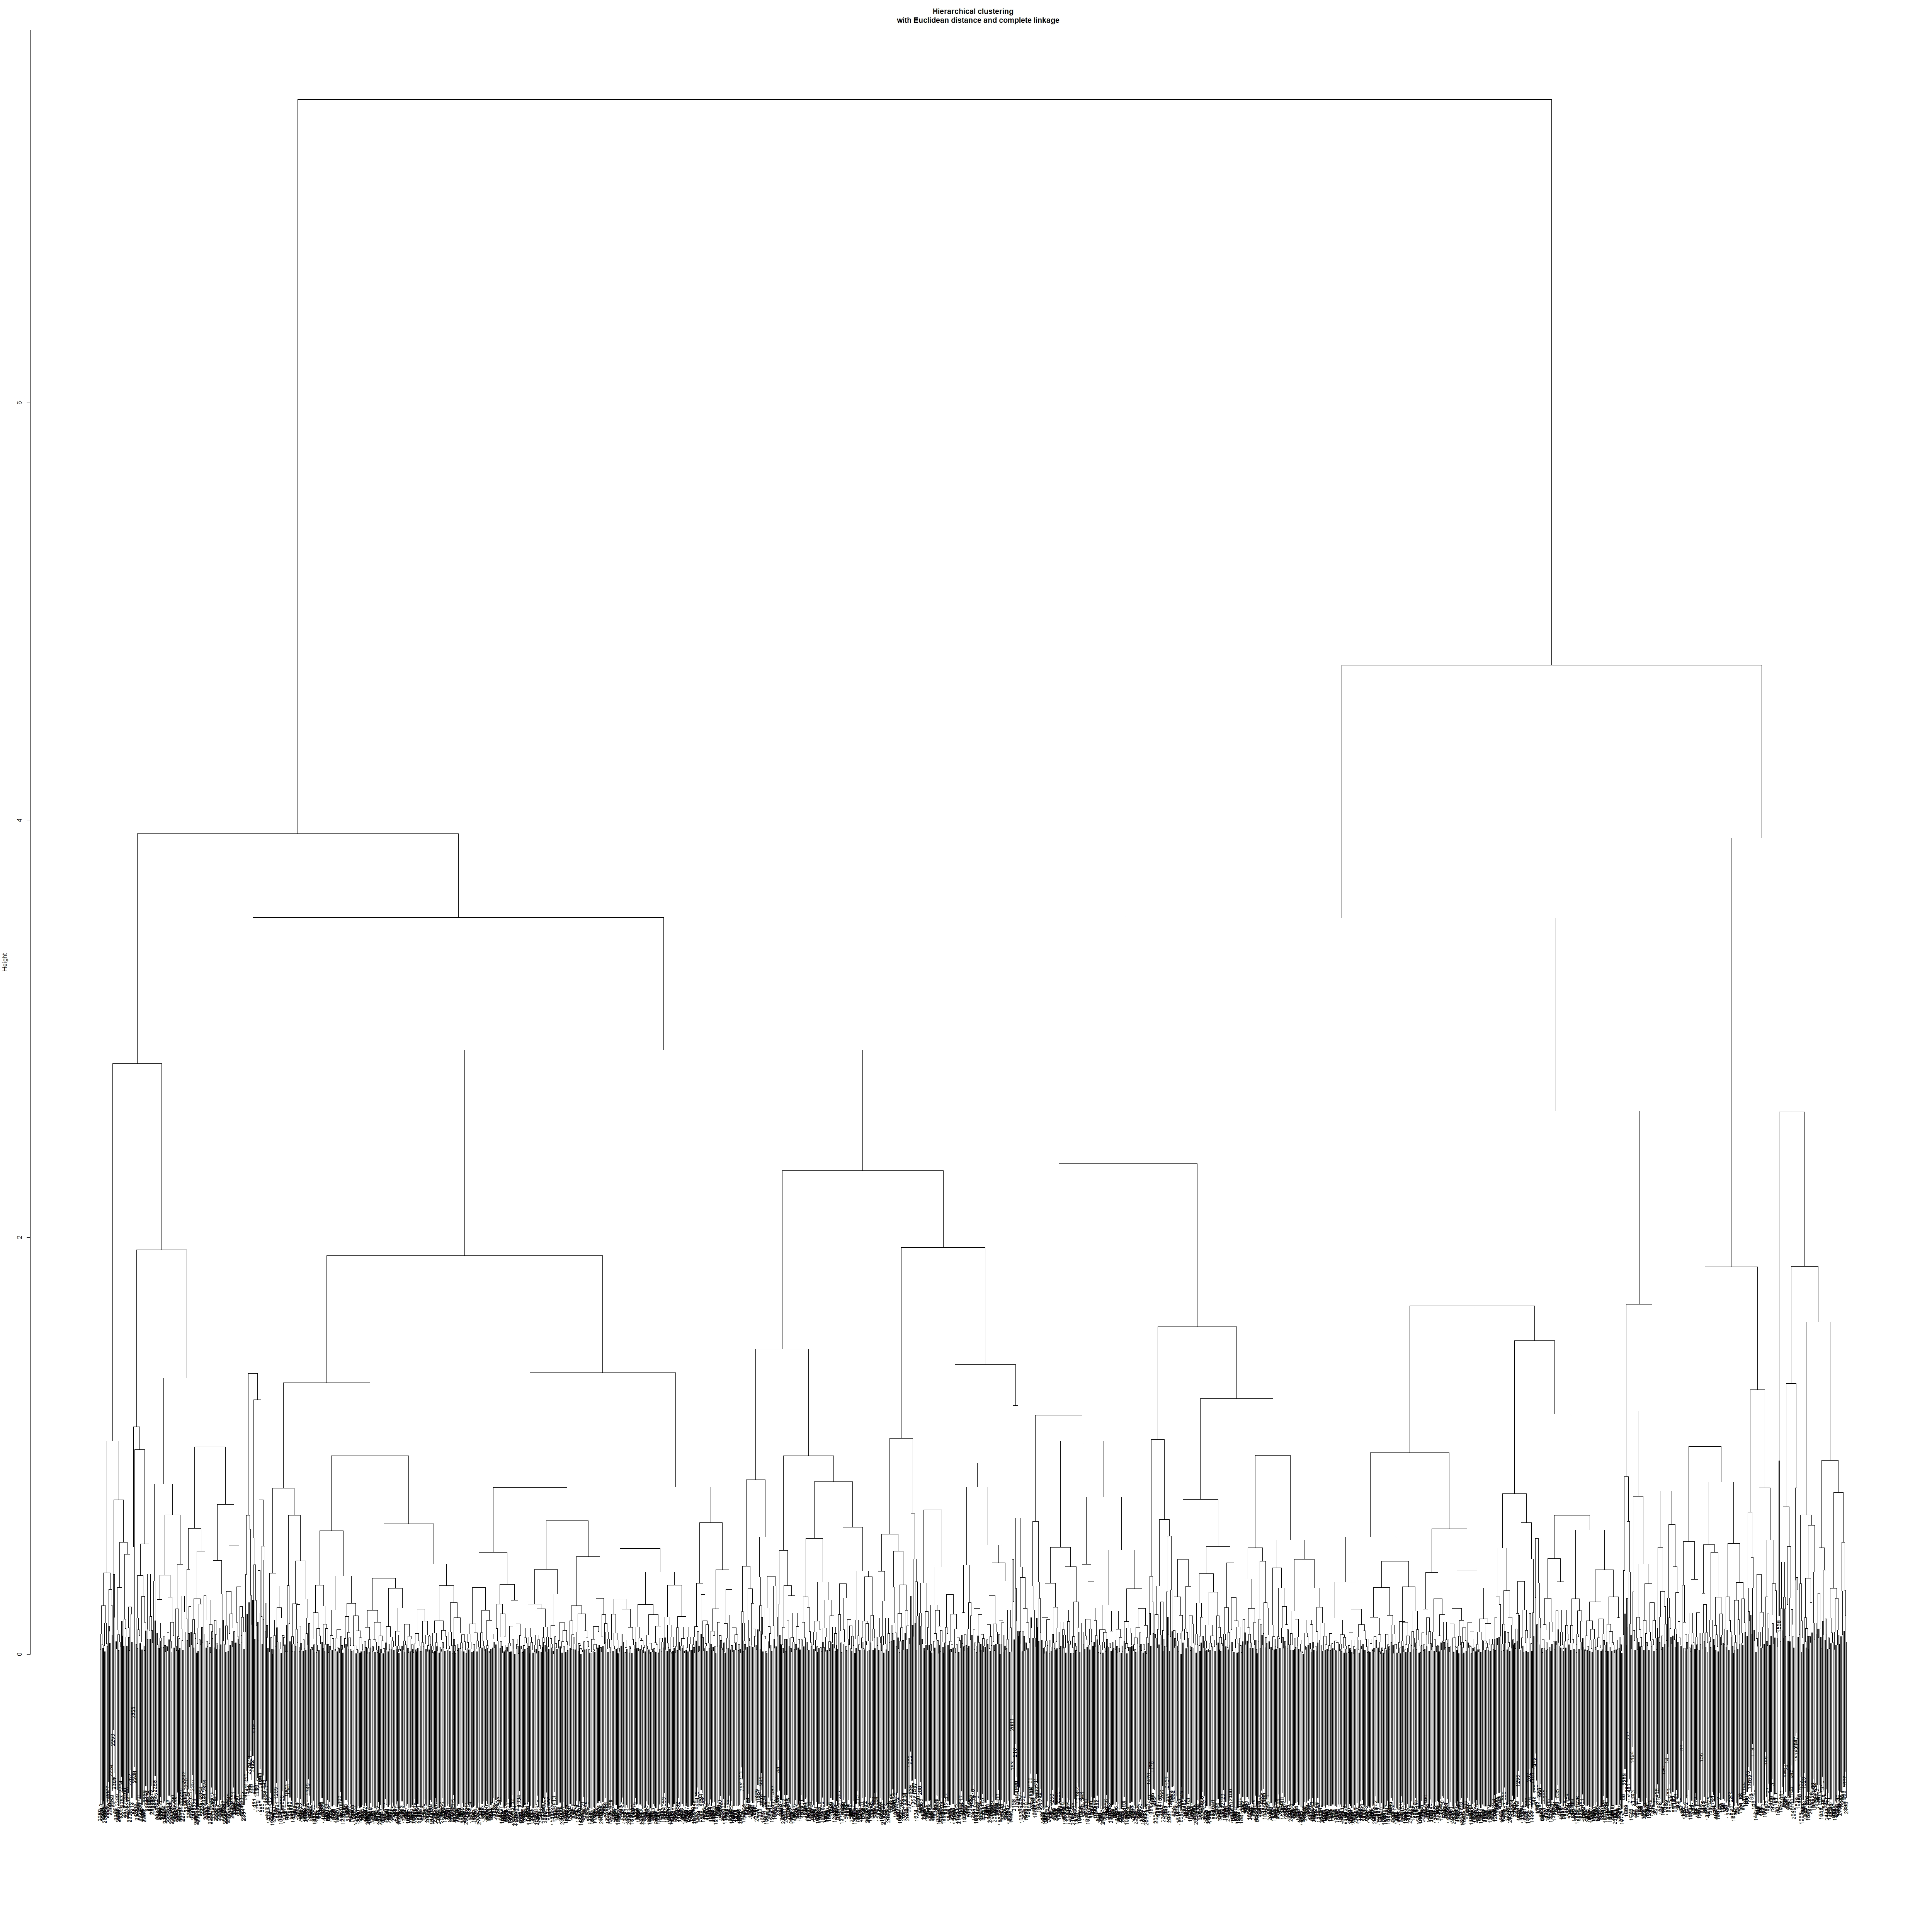
\includegraphics[width=9cm,height=9cm]{p32a.jpeg}
  \caption{Hierarchical clustering with Euclidean distance and complete linkage}
\end{figure}
\begin{figure}[H]
  \centering
  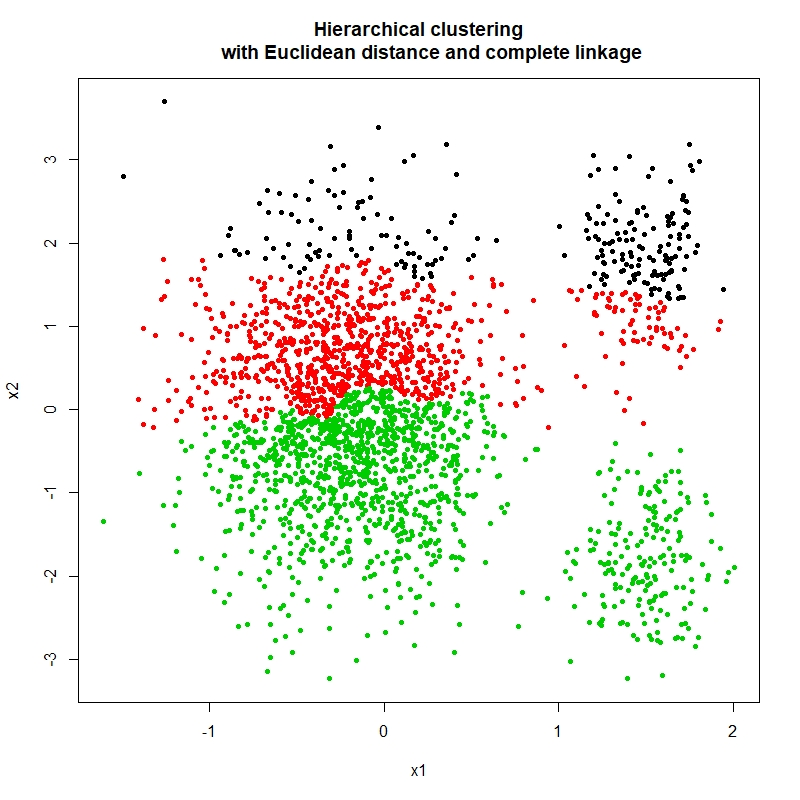
\includegraphics[width=9cm,height=9cm]{p32b.jpeg}
  \caption{Hierarchical clustering with Euclidean distance and complete linkage}
\end{figure}
\lstinputlisting{p32b.txt}
\begin{figure}[H]
  \centering
  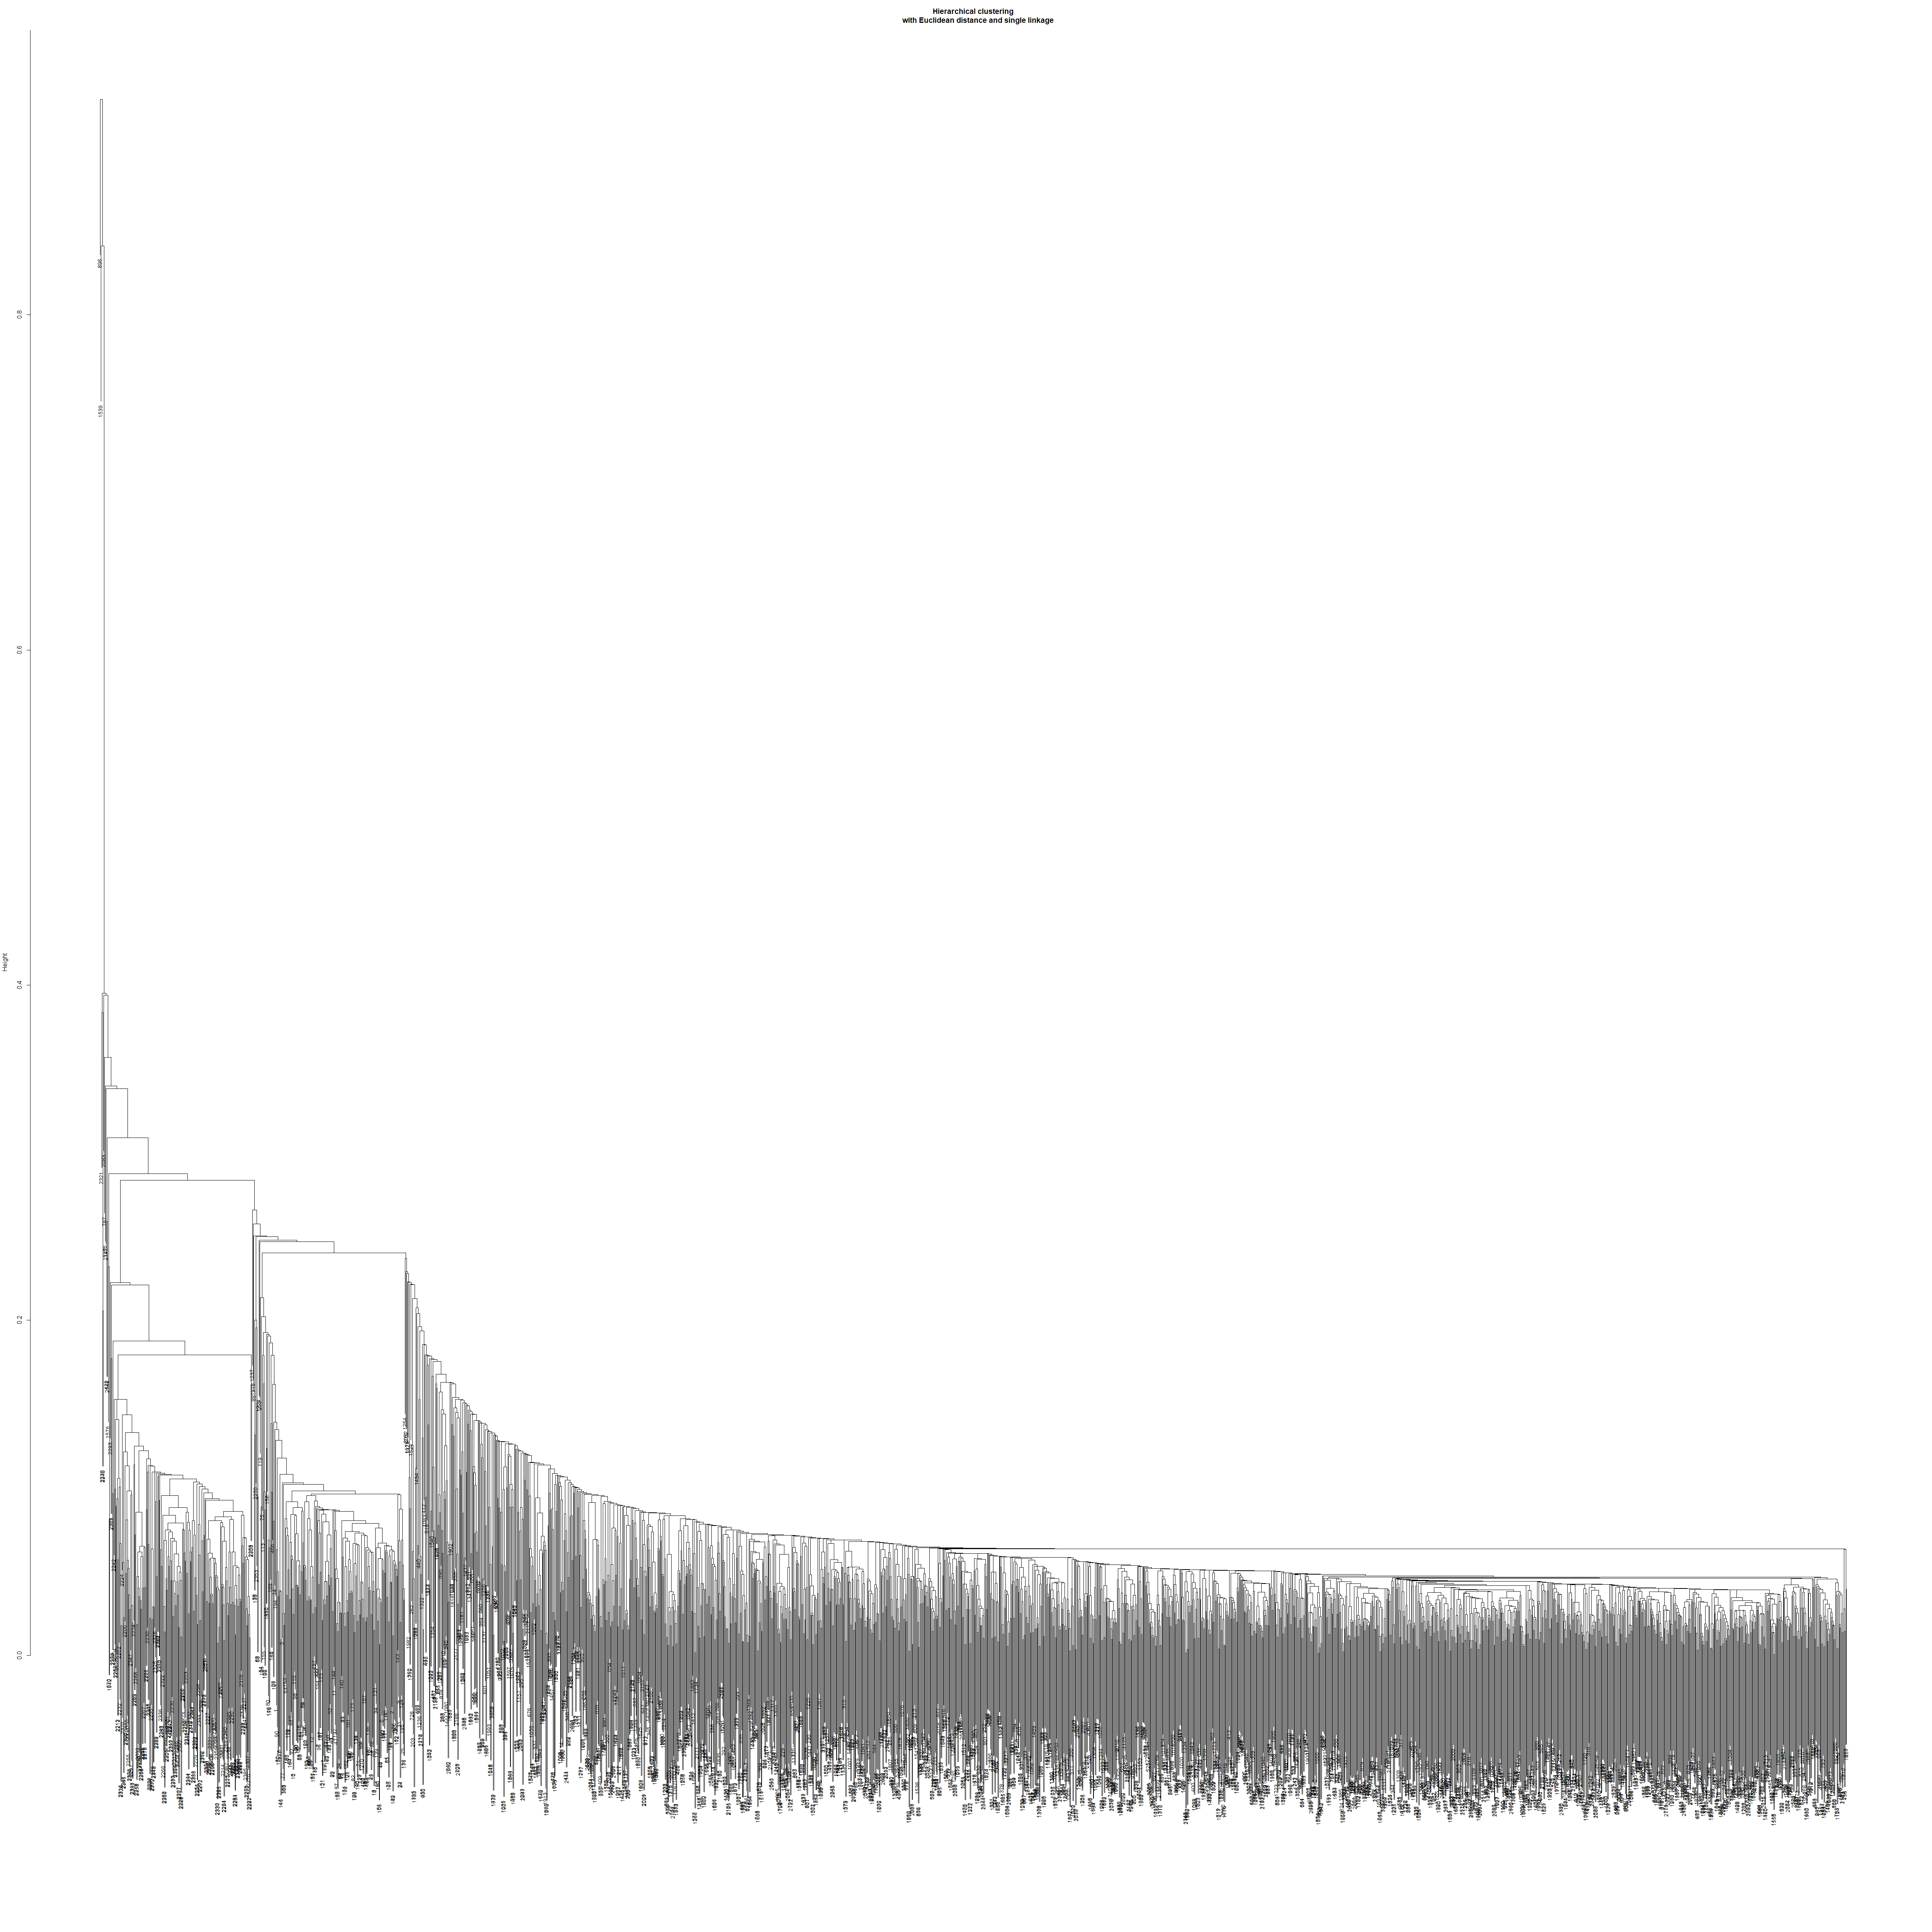
\includegraphics[width=9cm,height=9cm]{p32c.jpeg}
  \caption{Hierarchical clustering with Euclidean distance and single linkage}
\end{figure}
\begin{figure}[H]
  \centering
  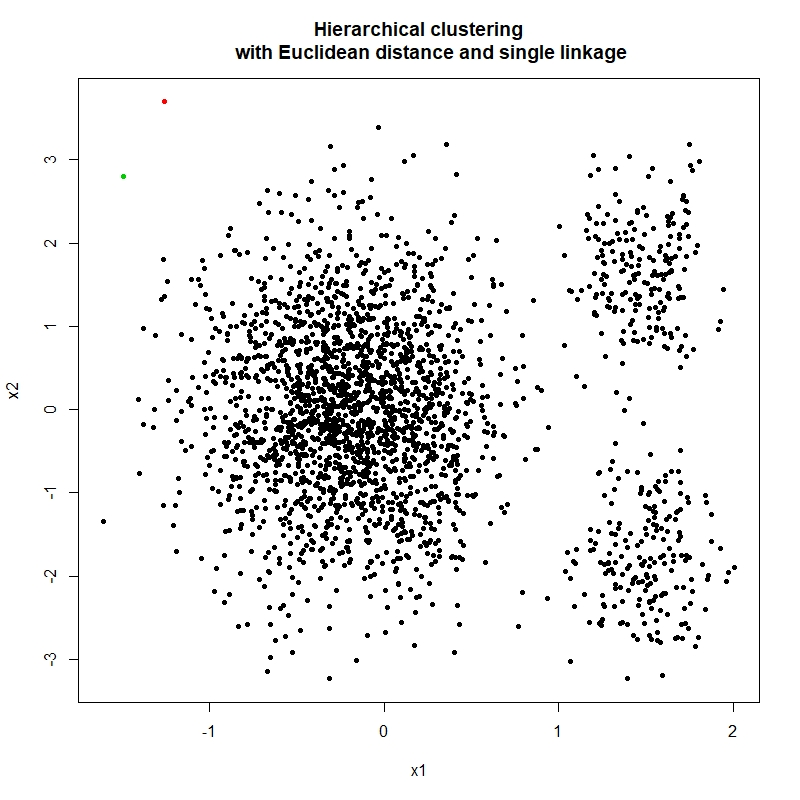
\includegraphics[width=9cm,height=9cm]{p32d.jpeg}
  \caption{Hierarchical clustering with Euclidean distance and single linkage}
\end{figure}
\vspace{3mm}

\item
R outputs:
\lstinputlisting{p33a.txt} % Comment: not needed

Comments:\\
The confusion matrices above show the accuracy of the K-means clustering ($K=3$) is 0.2533333; the accuracy of the hierarchical clustering with Euclidean distance and complete linkage is 0.48125; the accuracy of the hierarchical clustering with Euclidean distance and single linkage is 0.08375. The precision of the hierarchical clustering with Euclidean distance and complete linkage is the best of the three.\\
None of the three methods provides the similar clustering to the actual clustering in the data set. So, the outputs of the three are not ideal.\\
The hierarchical clustering with Euclidean distance and single linkage provides the worst clustering. Two outter points are clustered in two classes respectively and the rest of the points are clustered in one class.\\
The hierarchical clustering with Euclidean distance and complete linkage provides fine clustering. But many ``2'' points are misclustered as ``3'', a few ``2'' points are as ``1'', and a few ``1'' points are as ``2''.\\
The K-means clustering ($K=3$) provides fine clustering. But many ``2'' points are misclustered as ``1'' and a few ``2'' points are as ``3''.
\vspace{3mm}

Explanations:\\
Insights are shown in the confusion matrices and the accuracy of the each method. Please see the comments above.\\
The K-means clustering minimizes the within-cluster variation. It produces clusters with uniform sizes (each cluster with roughly an equal quantity of observations), even though the data might behave in a different way, and it is very sensitive to outliers and noisy data. Hence, we get three types of points in rougly equal amounts.\footnote{ Yse, D. L. (2019). \textit{A complete guide to K-means clustering algorithm}. Retrieved from \url{https://www.kdnuggets.com/2019/05/guide-k-means-clustering-algorithm.html}.}\\
The hierarchical clustering is based on tree-based graph. The complete linkage maximizes the distance (dissimilarity) between any
two observations in two different clusters, and the single linkage minimizes it. In this case, since the three acutal clusters have significant distances away from the other two, the maximizing strategy works well but the minimizing strategy works terribly.
\vspace{3mm}

\item
R codes:
\lstinputlisting{p34a.R}
R outputs:
\lstinputlisting{p34a.txt}
\begin{figure}[H]
  \centering
  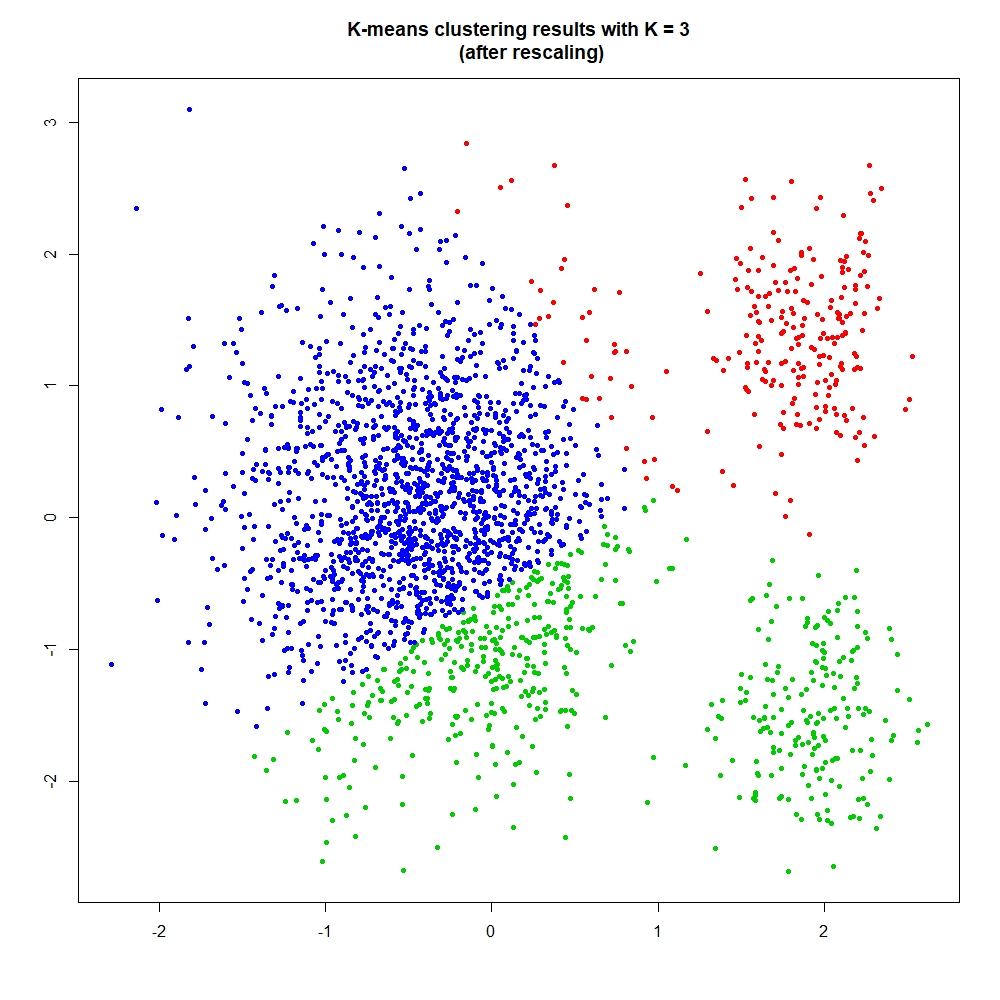
\includegraphics[width=9cm,height=9cm]{p34a.jpeg}
  \caption{K-means clustering results ($K=3$) (after rescaling)}
\end{figure}
\lstinputlisting{p34b.txt}
\begin{figure}[H]
  \centering
  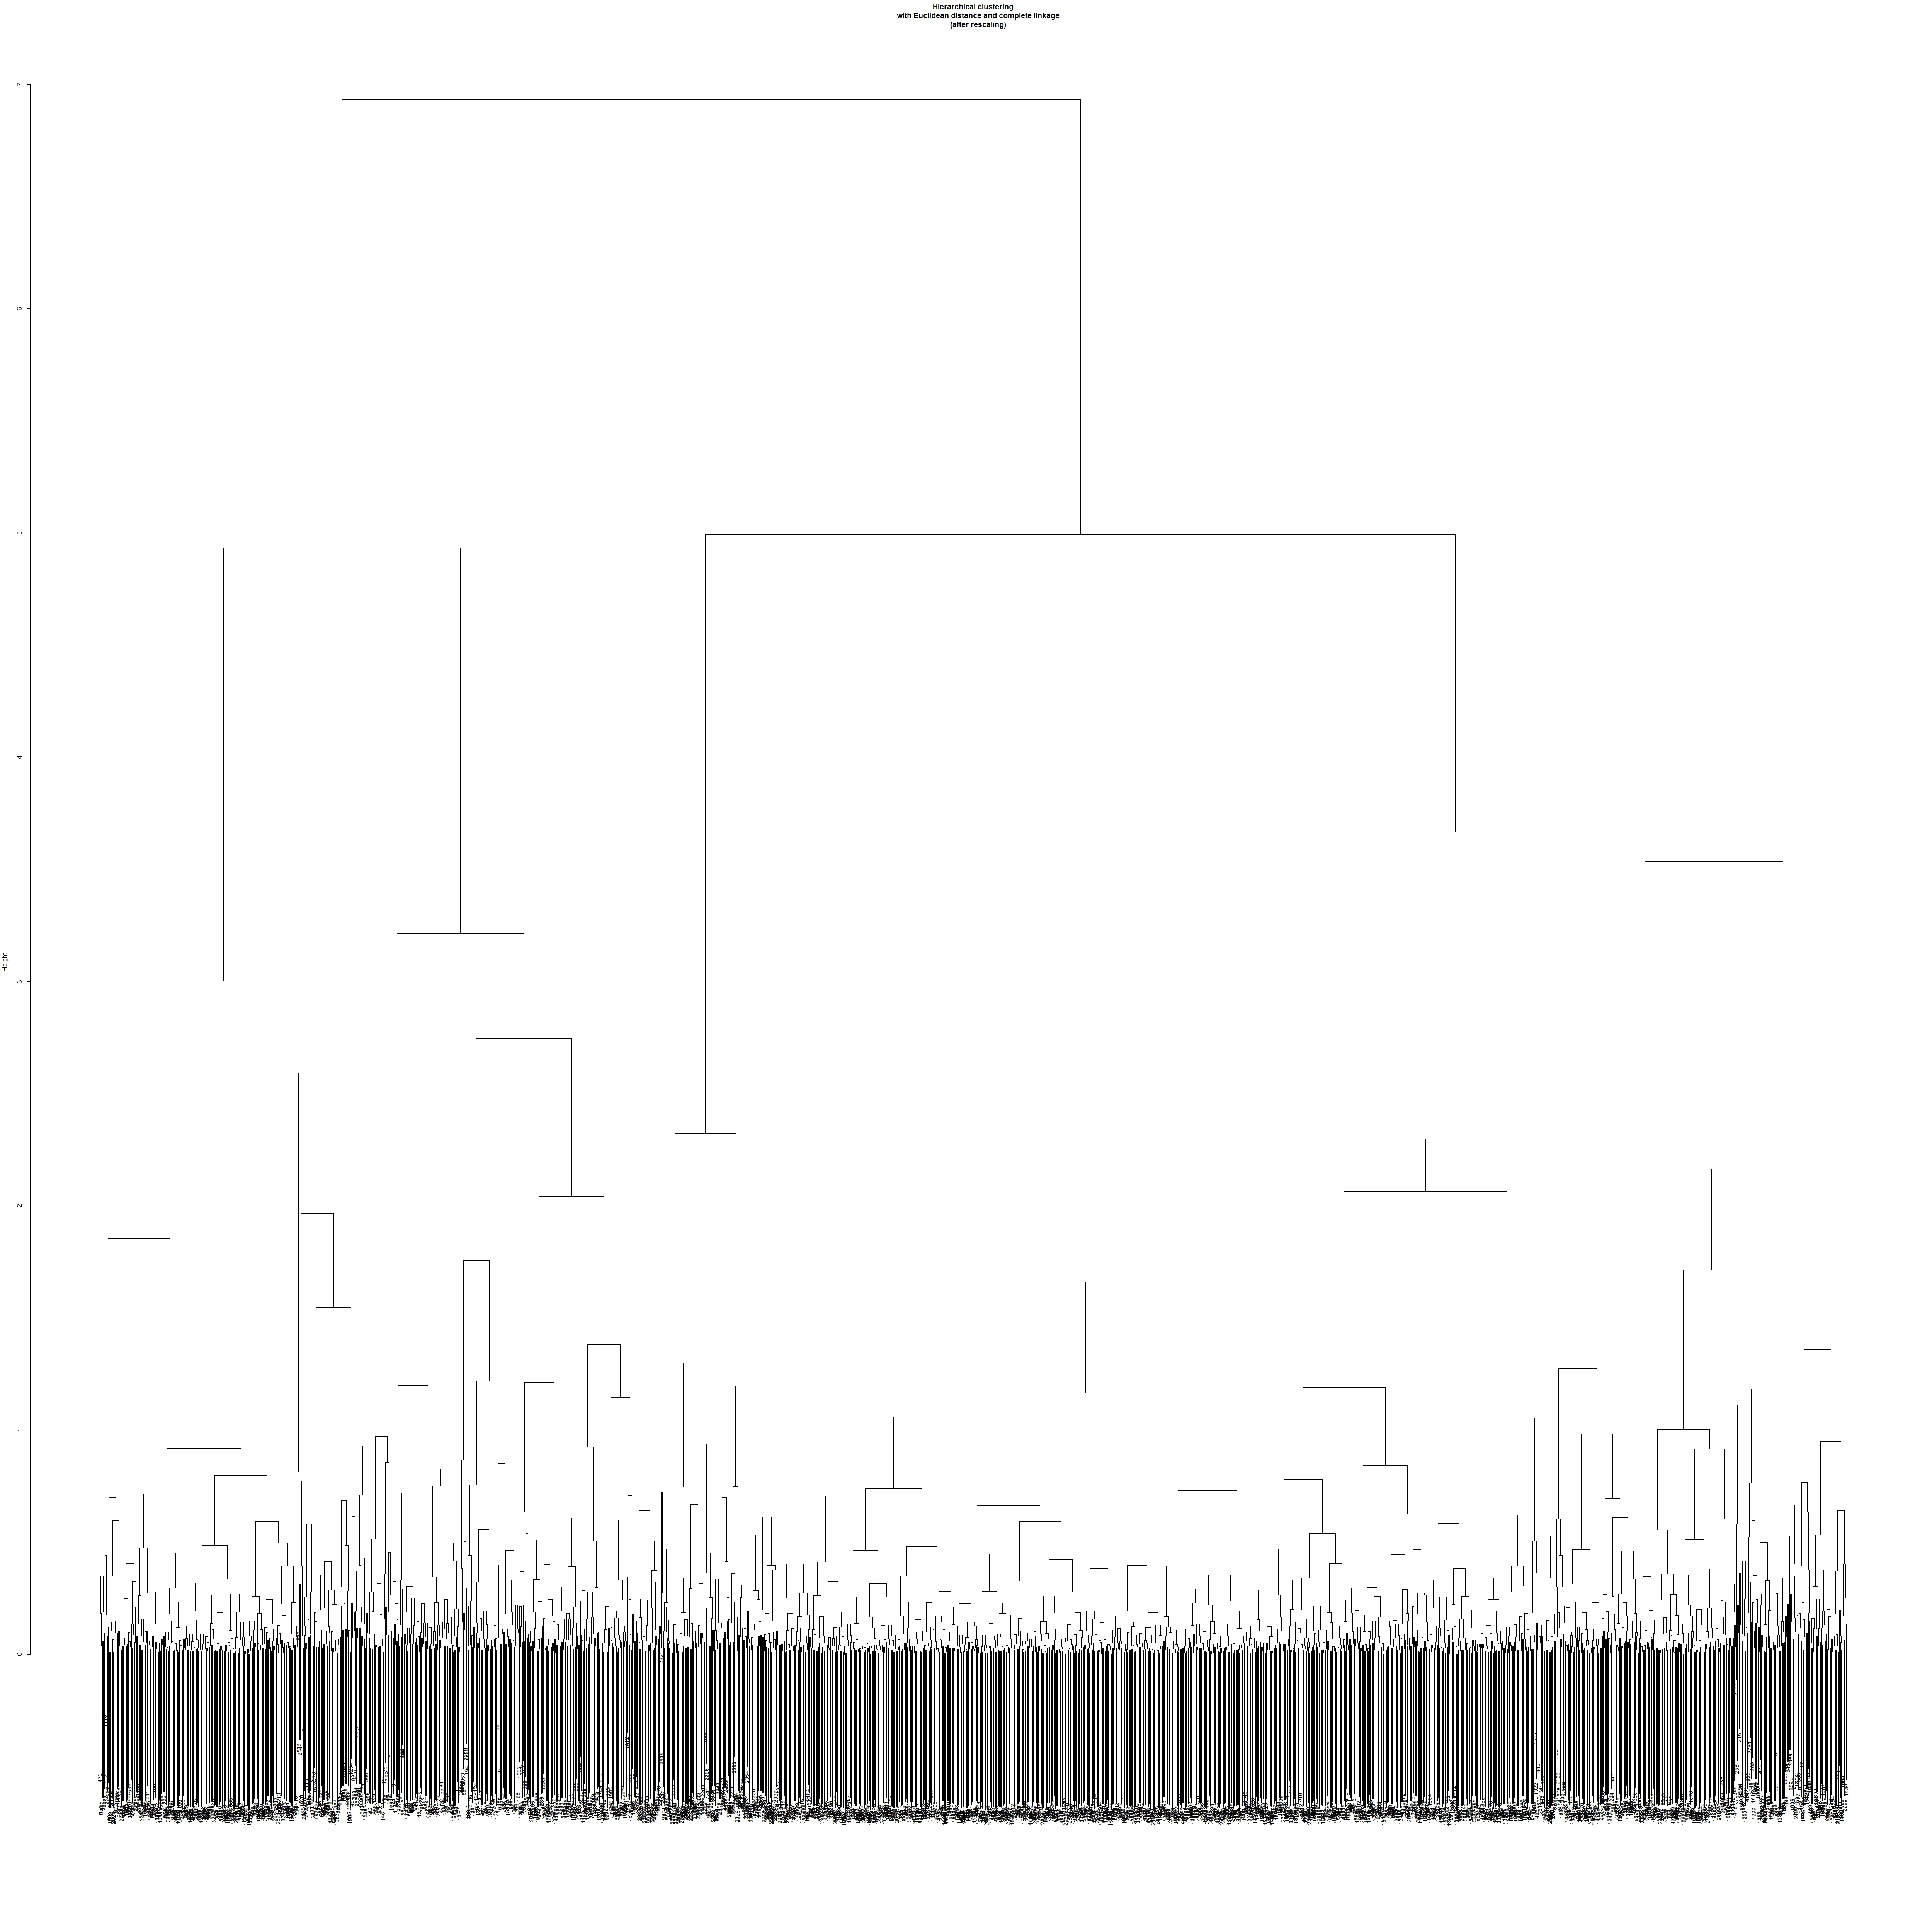
\includegraphics[width=9cm,height=9cm]{p34b.jpeg}
  \caption{Hierarchical clustering with Euclidean distance and complete linkage (after rescaling)}
\end{figure}
\begin{figure}[H]
  \centering
  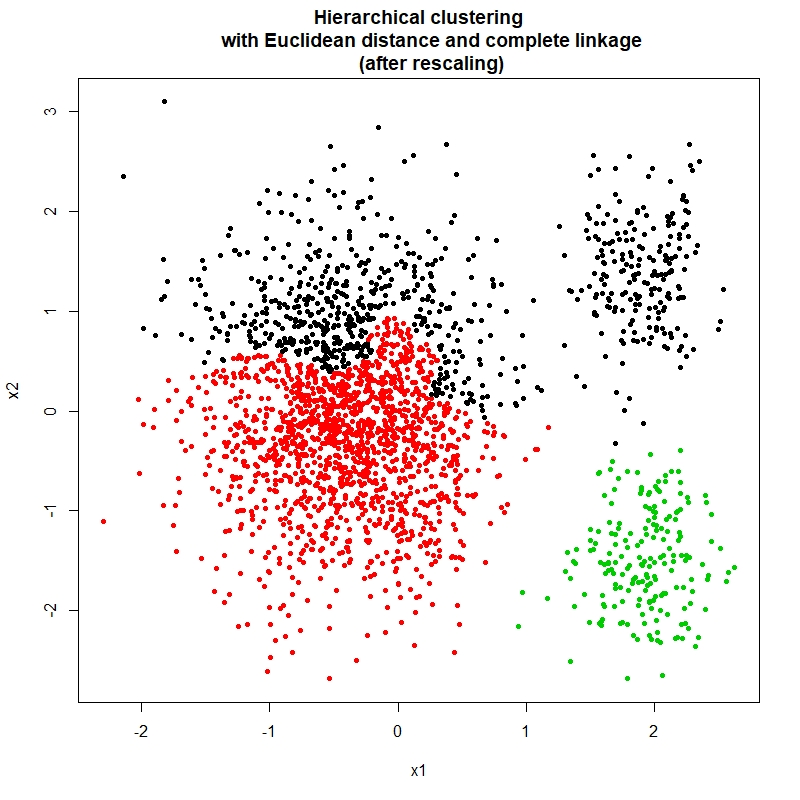
\includegraphics[width=9cm,height=9cm]{p34c.jpeg}
  \caption{Hierarchical clustering with Euclidean distance and complete linkage (after rescaling)}
\end{figure}
\lstinputlisting{p34c.txt}
\begin{figure}[H]
  \centering
  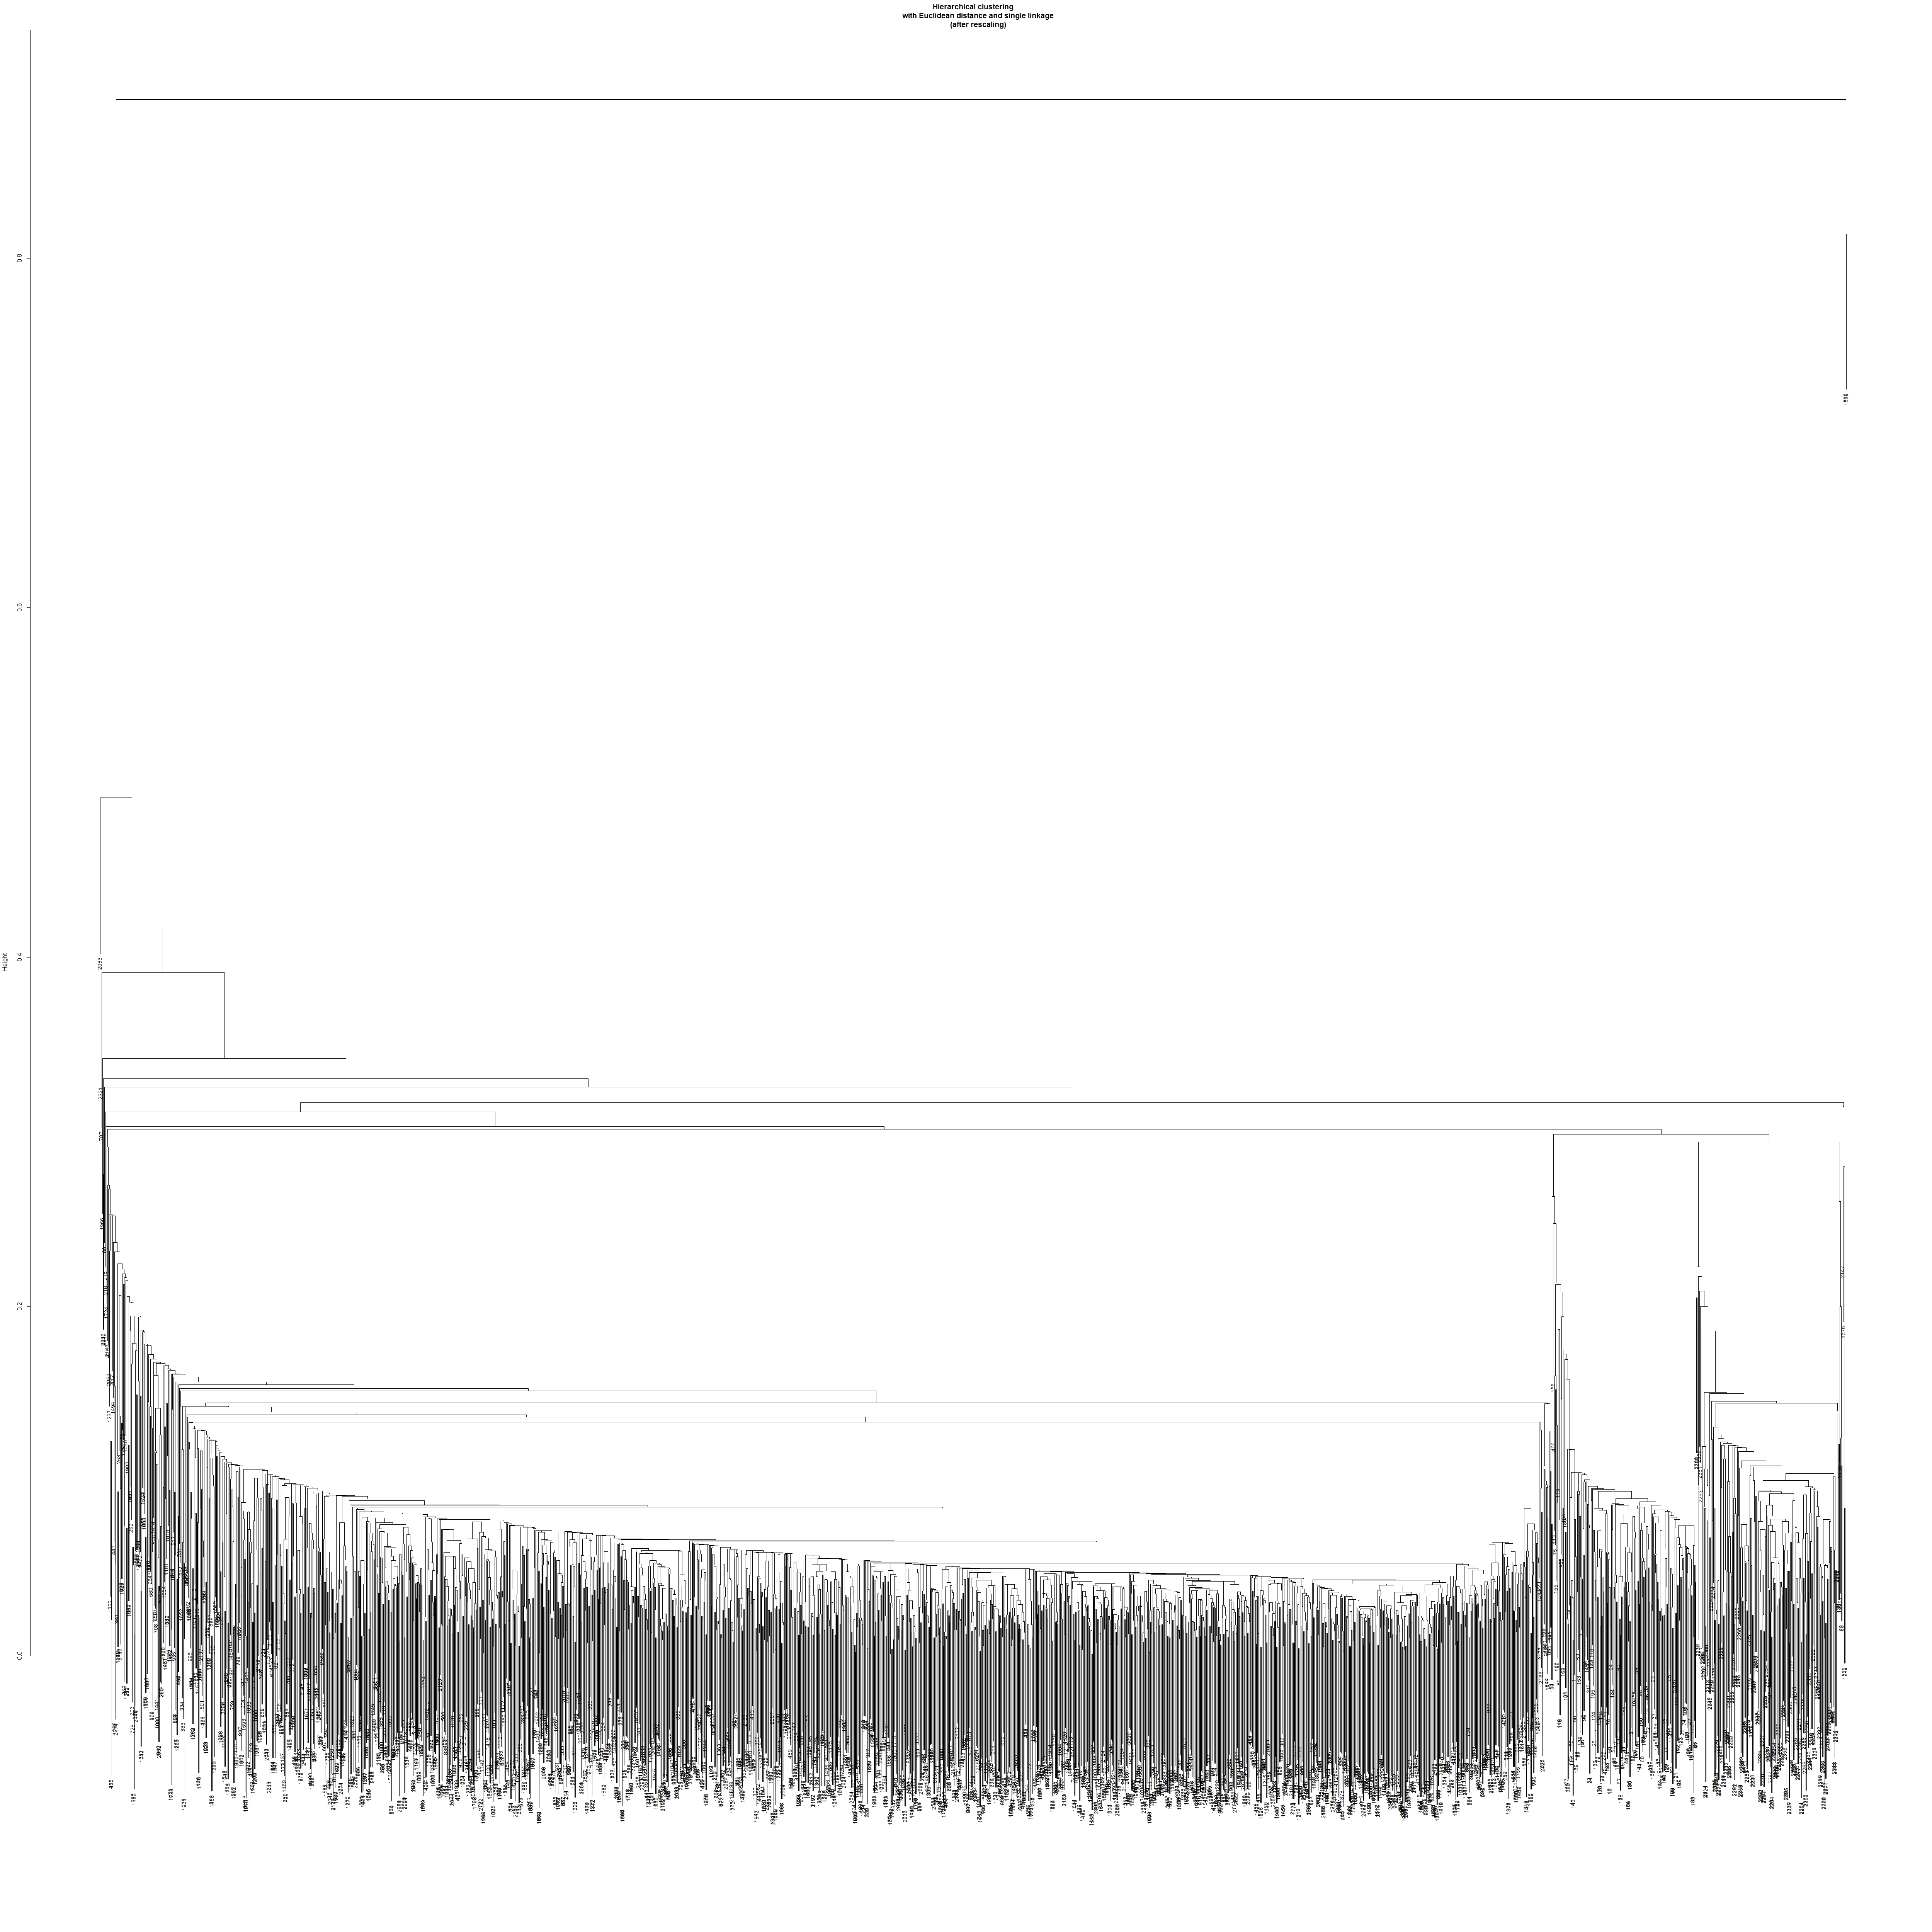
\includegraphics[width=9cm,height=9cm]{p34d.jpeg}
  \caption{Hierarchical clustering with Euclidean distance and single linkage (after rescaling)}
\end{figure}
\begin{figure}[H]
  \centering
  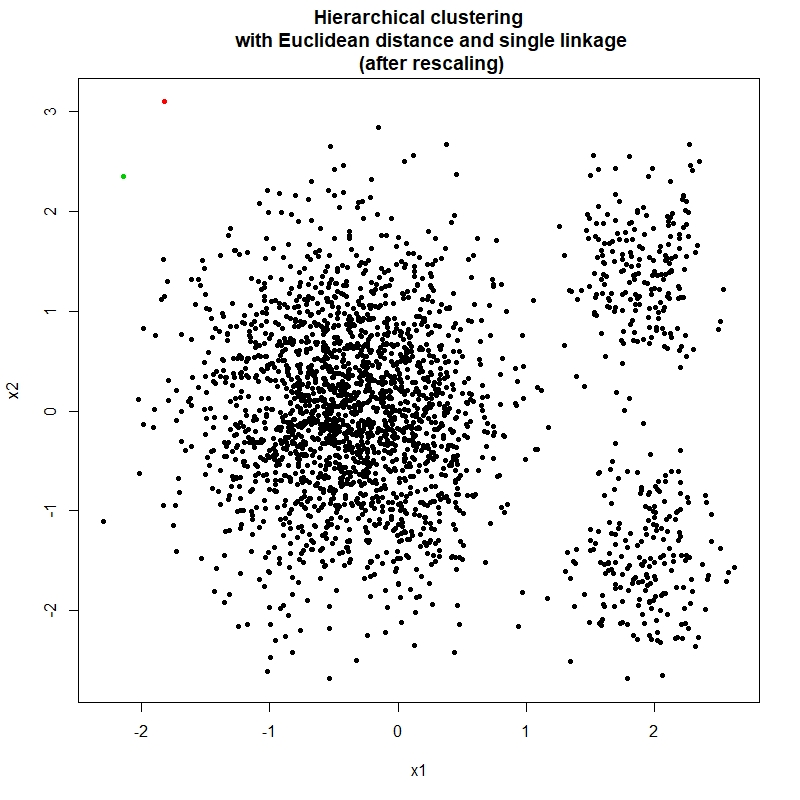
\includegraphics[width=9cm,height=9cm]{p34e.jpeg}
  \caption{Hierarchical clustering with Euclidean distance and single linkage (after rescaling)}
\end{figure}
\lstinputlisting{p34d.txt}
Does rescaling improve our results?\\
Yes for the K-means clustering ($K=3$) and the hierarchical clustering with Euclidean distance and complete linkage; no for the precision of the hierarchical clustering with Euclidean distance and single linkage.
\vspace{3mm}

Comments:\\
The confusion matrices above show the accuracy of the K-means clustering ($K=3$) is 0.48125, improved; the accuracy of the hierarchical clustering with Euclidean distance and complete linkage is 0.7754167, improved; the accuracy of the hierarchical clustering with Euclidean distance and single linkage is 0.08375, not improved. The precision of the hierarchical clustering with Euclidean distance and complete linkage is the best of the three.\\
The hierarchical clustering with Euclidean distance and single linkage does not get improved.\\
The hierarchical clustering with Euclidean distance and complete linkage gets improved. Almost all the ``1'' and ``3'' points are correctly clustrered. But more ``2'' points were misclustered as ``1'' comparing to the outputs before rescaling.\\
The K-means clustering gets more improved. Almost all the ``1'' and ``3'' points are correctly clustrered, and the ``2'' points that were misclusttered as ``1'' get less. The points ``2'' misclustered as ``3'' increase a bit. % Comment: x
\vspace{3mm}

Explanations:\\
Insights are shown in the confusion matrices and the accuracy of the each method. Please see the comments above.\\
Since x1 and x2 may have different meanings and magnitudes, the scaling works. Methods with an Euclidean distance measure is sensitive to magnitudes and hence scaling can improve the outputs. But since the difference in magnitudes of the data is small, there is no significant change for the single linkage method. However, for the complete linkage method and the K-mean method, the scaling changes the outputs.
\vspace{3mm}

\end{enumerate}
\vspace{3mm}

\begin{prob}
\end{prob}
\begin{enumerate}[1)]
\vspace{3mm}

\item
R codes:
\lstinputlisting{p41a.R}
R outputs:
\begin{figure}[H]
  \centering
  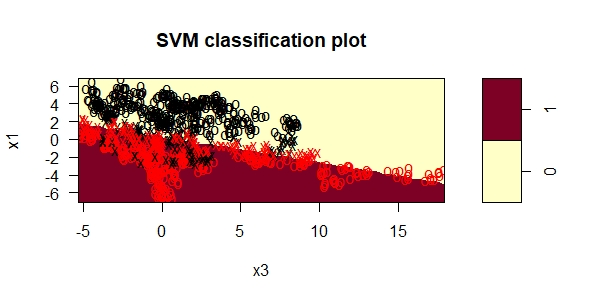
\includegraphics[width=10cm,height=5cm]{p41a.jpeg}
  \caption{SVM classification with cost = 10000}
\end{figure}
Yes, we can find a separating hyperplane using the svm() function in R, namely the linear separability.\footnote{ James, G., Witten, D., Hastie, T., \& Tibshirani, R. (2014). \textit{An introduction to statistical learning with applications in R}. Springer, 362.} We can use a large cost value, namely a narrow margine, to find the hyperplane shown above. % Comment: x
\vspace{3mm}

\item
R codes:
\lstinputlisting{p42a.R}
R outputs:
\lstinputlisting{p42a.txt}
We get the best cost value $10$.\\
R outputs:
\begin{figure}[H]
  \centering
  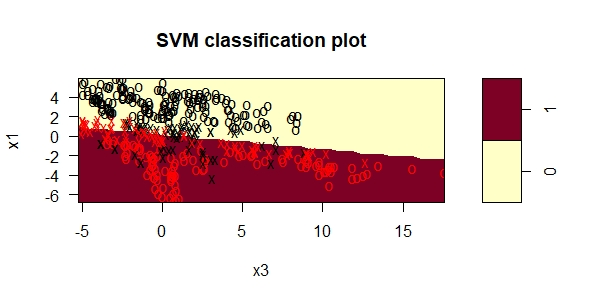
\includegraphics[width=10cm,height=5cm]{p42a.jpeg}
  \caption{SVM classification with cost = 10}
\end{figure}
\lstinputlisting{p42b.txt}
\vspace{3mm}
The confusion matrix:\\
\begin{tabular}{llllll}
                                          &         & \multicolumn{2}{l}{True Banknote Type} &       &  \\
                                          &         & Genuine           & Forged             & Total &  \\
\multirow{2}{*}{Predicted Banknote Types} & Genuine & 207               & 29                 & 236   &  \\
                                          & Forged  & 11                & 165                & 176   &  \\
                                          & Total   & 218               & 194                & 412   &
\end{tabular}
\vspace{3mm}

Comments:\\
The testing error rate is 0.0971 ($=(11+29)/412$).\\
The accuracy is 0.9029; the misclassification rate is 0.0971.\\
The true positive rate is 0.8505 ($=165/194$); the false positive rate is 0.0505 ($=11/218$).\\
The true negative rate is 0.9495 ($=207/218$); the false negative rate is 0.1495 ($=29/194$).\\
The precision is 0.9375 ($=165/176$), being acceptable; the specificity is 0.9495 ($=1-11/218$), being acceptable; the sensitivity is 0.8505 ($=1-29/194$), being acceptable.\\
The tune() function recommends different best costs when excuted.
\vspace{3mm}

\item
R codes:
\lstinputlisting{p43a.R}
R outputs:
\lstinputlisting{p43a.txt}
We get the best cost value $10$ and the best gamma value $4$.\\
R outputs:
\begin{figure}[H]
  \centering
  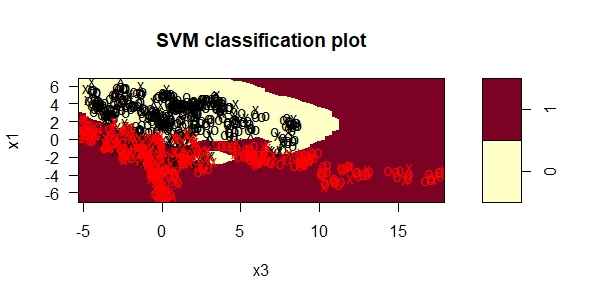
\includegraphics[width=10cm,height=5cm]{p43a.jpeg}
  \caption{SVM classification with the radial kernel, cost = 10 and gamma = 4}
\end{figure}
\lstinputlisting{p42b.txt}
\vspace{3mm}
The confusion matrix:\\
\begin{tabular}{llllll}
                                          &         & \multicolumn{2}{l}{True Banknote Type} &       &  \\
                                          &         & Genuine           & Forged             & Total &  \\
\multirow{2}{*}{Predicted Banknote Types} & Genuine & 212               & 24                 & 236   &  \\
                                          & Forged  & 12                & 164                & 176   &  \\
                                          & Total   & 224               & 188                & 412   &
\end{tabular}
\vspace{3mm}

Comments:\\
The testing error rate is 0.0874 ($=(12+24)/412$).\\
The accuracy is 0.9126; the misclassification rate is 0.0874.\\
The true positive rate is 0.8777; the false positive rate is 0.0536.\\
The true negative rate is 0.9464; the false negative rate is 0.1276.\\
The precision is 0.9318, being acceptable; the specificity is 0.9464, being acceptable; the sensitivity is 0.8723, being acceptable.
\vspace{3mm}

Compare our results with those obtained in part (b):\\
For the outputs with the radial kernel, cost = 10 and gamma = 4, the testing error rate decreases; the accuracy is increases; the precision decreases; the specificity decreaseas; the sensitivity increases. The changes are not significant and this SVM slightly gets better.

\end{enumerate}
\vspace{3mm}

\end{document}